\newcommand*{\Root}{..}
\documentclass[12pt,a4paper]{report}
\usepackage[utf8]{inputenc}
\usepackage[toc,page]{appendix}
\usepackage[english]{babel}
\usepackage[margin=1in]{geometry}
\usepackage[pdftex]{graphicx}
\usepackage{biblatex}
\usepackage{caption}
\usepackage{hyperref}
\usepackage{listing}
\usepackage{listings,lstautogobble}
\usepackage[default,scale=0.95]{opensans}
\usepackage{scrlayer}
\usepackage{setspace}
\usepackage[caption=false]{subfig}
\usepackage{titlesec}
\usepackage{xcolor}

% Custom colors
\definecolor{code-background}{HTML}{EEEEEE}
\definecolor{code-delim}{RGB}{20,105,176}
\colorlet{code-punct}{red!60!black}

% Custom English translations.
\addto\extrasenglish{%
	\def\subsubsectionautorefname{section}%
}

% Configuration for code listings.
\lstdefinelanguage{json}{
	basicstyle=\normalfont\ttfamily,
	numbers=left,
	numberstyle=\scriptsize,
	stepnumber=1,
	numbersep=8pt,
	showstringspaces=false,
	breaklines=true,
	frame=lines,
	backgroundcolor=\color{code-background},
	literate=
	*{:}{{{\color{code-punct}{:}}}}{1}
	{,}{{{\color{code-punct}{,}}}}{1}
	{\{}{{{\color{code-delim}{\{}}}}{1}
	{\}}{{{\color{code-delim}{\}}}}}{1}
	{[}{{{\color{code-delim}{[}}}}{1}
	{]}{{{\color{code-delim}{]}}}}{1},
}


\newcommand\YAMLcolonstyle{\color{red}\mdseries}
\newcommand\YAMLkeystyle{\color{black}\bfseries}
\newcommand\YAMLvaluestyle{\color{blue}\mdseries}

\makeatletter

% here is a macro expanding to the name of the language
% (handy if you decide to change it further down the road)
\newcommand\language@yaml{yaml}

\expandafter\expandafter\expandafter\lstdefinelanguage
\expandafter{\language@yaml}
{
	keywords={true,false,null,y,n},
	keywordstyle=\color{darkgray}\bfseries,
	basicstyle=\YAMLkeystyle,                                 % assuming a key comes first
	sensitive=false,
	comment=[l]{\#},
	morecomment=[s]{/*}{*/},
	commentstyle=\color{purple}\ttfamily,
	stringstyle=\YAMLvaluestyle\ttfamily,
	moredelim=[l][\color{orange}]{\&},
	moredelim=[l][\color{magenta}]{*},
	moredelim=**[il][\YAMLcolonstyle{:}\YAMLvaluestyle]{:},   % switch to value style at :
	morestring=[b]',
	morestring=[b]",
	literate =    {---}{{\ProcessThreeDashes}}3
	{>}{{\textcolor{red}\textgreater}}1     
	{|}{{\textcolor{red}\textbar}}1 
	{\ -\ }{{\mdseries\ -\ }}3,
}


\lstset{
	numbers=left,
	numberstyle=\scriptsize,
	stepnumber=1,
	numbersep=8pt,
	showstringspaces=false,
	breaklines=true,
	frame=lines,
	backgroundcolor=\color{code-background},
	autogobble=true
}

\titleclass{\chapter}{straight}

\titleformat{\chapter}[display]{\normalfont\huge\bfseries}{\chaptertitlename\ \thechapter}{18pt}{\huge}
\titlespacing*{\chapter}{0pt}{20pt}{20pt}

\setcounter{secnumdepth}{5}

% Default values for variables.
\newcommand{\documentdate}{\today}
\newcommand{\documenttitle}{Undefined "documenttitle"}

% Custom macros.
\newcommand{\bolditem}[1]{\item \textbf{#1:}}
\begin{document}
\DeclareNewLayer[
foreground,
foot,
contents={\parbox[b][\layerheight][b]{\layerwidth}{%
		
\includegraphics[height=2.5cm]{\Root/.latex-common/logo-ghent-university.pdf}
		\hfill
		
\includegraphics[height=1.2cm]{\Root/.latex-common/logo-sciences.pdf}%
		\vspace*{1cm}
}}
]{titlepage.logos}

\title{
	\vspace*{1.4in}
	\Huge{Thesis (working draft)}\\
	\vspace*{0.4in}
	\Large{\documenttitle}\\
	\vspace*{4cm}
}

\date{\documentdate}
\author{Pieter De Clercq\vspace*{3.5cm}}

\AddLayersToPageStyle{empty}{titlepage.logos}
\maketitle
\RemoveLayersFromPageStyle{empty}{titlepage.logos}
\onehalfspacing
\newpage

\chapter*{Metadata}
\emph{The title of my thesis is still provisionary as I have slightly adapted my subject (see the Status-section).}

\begin{itemize}
  \item \textbf{Title:} Reducing the cost and duration of Continuous Integration
  \item \textbf{Name:} Pieter De Clercq \texttt{(01503338)}
  \item \textbf{Study programme:} Master of Science in Computer Science
  \item \textbf{Promotor(s):} prof. dr. Bruno Volckaert, prof. dr. ir. Filip De Turck
  \item \textbf{Supervisors:} Jasper Vaneessen, Dwight Kerkhove
\end{itemize}

\chapter*{Status}
Back in February-March when I had proposed my subject on Continuous Integration, I was given the advice to choose my subject as broad as possible and then refine it during my literature study. My original idea was to perform research into the distribution and scalability of Continous Integration systems, on constrained (low-end) devices. On the first meeting with my supervisors, I was tasked with identifying common problems on this subject in order to determine the scope of my thesis. While performing this research however, I quickly discovered a more interesting problem, which is related to scalability but in a slightly different way.\\

\noindent Currently one of the major issues with Continuous Integration is the following: In software, a \emph{regression} is defined as a part of the software that initially was working and then broke, for example because of a change in the codebase. In order to fix this, the developer typically writes a \emph{regression test}. This test should fail, because the part it intends to test is broken, and the developer should resolve the broken part in order to make the test pass. It is clear that a regression test can never be removed from the test suite, because this could possibly cause that same bug to reoccur at some point in the future. As time goes on, this results in a large test suite, which needs to be fully executed every single time a developer contributes work to the project. In this thesis I want to research whether it is possible to predict which tests will fail, give(n a certain change in the code, in order to execute the tests with the highest probability of failling as soon as possible. This saves developers multiple hours of waiting for CI results, as they can start identifying and resolving issues sooner if a test already fails in the beginning of the test suite.\\

\noindent After I had identified this problem, I have found and read several research papers on this subject. Every paper describes approaches to determine whether or not a test might fail. Next, I have searched for open-source projects, that also publicize their build data. Currently I have found two Java projects (REST-assured\footnote{\url{https://rest-assured.io/}} and Mockito\footnote{\url{https://site.mockito.org/}}. Additionally, I have also included Dodona\footnote{\url{https://dodona.ugent.be}}, a project started by my own faculty which is coded in Ruby-on-Rails, because I am very familiar with the codebase thanks to previous student jobs. For all three of these projects, I have identified the failing builds and wrote scripts to scrape and extract usable data by parsing the build logs, as can be seen in \autoref{fig:builds-pre} and \autoref{lst:builds-post}.

\begin{figure}[htbp]
  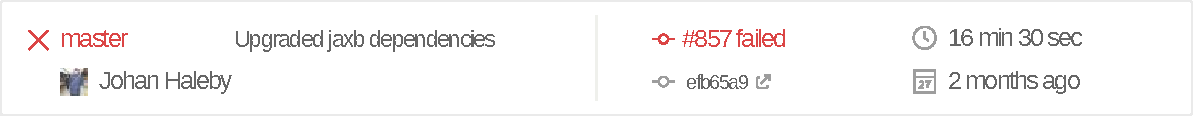
\includegraphics[width=\textwidth]{assets/builds-pre.pdf}
  \caption{Raw build data from Travis CI}
  \label{fig:builds-pre}
\end{figure}

\begin{lstlisting}[caption="Resulting JSON after parsing", label=lst:builds-post, language=json]
{
  "build": 580593658,
  "commit": "efb65a9110eb70462fe211fce1069995cf11615e",
  "job": 580593659,
  "failed_tests": [
    {
      "test": "urlEncodingDisabledStatically",
      "file": "io.restassured.itest.java.URLEncodingITest"
    }
  ],
  "changed_files": [
    { filename": "pom.xml", "status": "modified" }
  ],
  "parents": [
    "c81aa3ef21f320a2a61b4a10f9f8f5272433731e"
  ]
}
\end{lstlisting}

\chapter*{Schedule}
First of all, I will continue my search to find usable open-source projects, preferably large, active projects that have lots of failing builds. I was advised to consider projects such as Chromium, VLC and projects by the Apache Software Foundation, but these turn out to be non-trivial to use. The most prevalent problem is that either the builds hardly ever fail, or that the retention of the build log is very low (e.g. build logs are deleted after 5 days).\\

\noindent Then, I want to compile a list of all possible approaches (algorithms) that I can take to tackle the problem. Most of the papers I have read describe Machine Learning-based approaches, but some papers also describe simple yet efficient heuristics. Since I am not very proficient in Machine Learning, I will focus on the second category. The hardest part is determining which test is responsible for which part of the application source code. To accomplish this mapping, I want to look into the inner workings of code coverage tools and try to extract the required information, or write a custom simple coverage agent if this turns out to be unfeasible.\\

\noindent The final step will be to setup a simple Proof of Concept-architecture and write a full-text literature report, which will serve as the first part of my final thesis.

\chapter*{Remarks}
I am a parttime freelance developer. My last project was delivered on October 15th and I will not accept any new projects, so now I can dedicate all my time to my thesis.

\end{document}
